% Chapter 10, Section 1

\section{Recurrent Neural Networks}
\label{sec:rnns}
\difficulty{intermediate}

\subsection*{Intuition}

An RNN carries a running summary of the past—like a notepad you update after reading each word. This hidden state lets the model use prior context to influence current predictions. However, keeping reliable notes over long spans is hard: small errors can compound, and gradients may shrink or grow too much \cite{GoodfellowEtAl2016}.

\subsection*{Historical Context}

Early sequence models struggled with long-term dependencies due to vanishing gradients, motivating gated designs such as LSTM \cite{Hochreiter1997}. Practical training stabilized with techniques like gradient clipping and better initialization \cite{GoodfellowEtAl2016}.

% Index and glossary
\index{recurrent neural network}
\glsadd{recurrent-neural-network}

\subsection{Motivation}

Sequential data has temporal dependencies:
\begin{itemize}
    \item Time series (stock prices, sensor readings)
    \item Text (words depend on previous words)
    \item Speech (phonemes form words)
    \item Video (frames over time)
\end{itemize}

Standard feedforward networks cannot capture these dependencies effectively.

\subsection{Basic RNN Architecture}

An RNN maintains a hidden state $\vect{h}_t$ that evolves over time:

\begin{align}
\vect{h}_t &= \sigma(\mat{W}_{hh} \vect{h}_{t-1} + \mat{W}_{xh} \vect{x}_t + \vect{b}_h) \\
\vect{y}_t &= \mat{W}_{hy} \vect{h}_t + \vect{b}_y
\end{align}

where $\vect{x}_t$ is input at time $t$, and $\sigma$ is typically tanh.

\paragraph{Visual aid.} The following unrolled diagram shows shared parameters across time:
\begin{figure}[h]
    \centering
    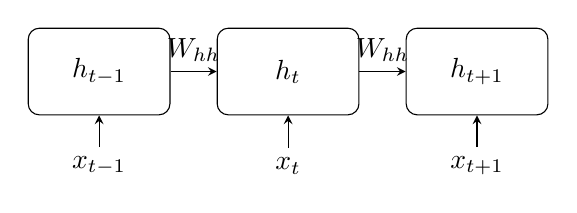
\begin{tikzpicture}[>=stealth, node distance=2.4cm]
        \tikzstyle{node}=[draw, rounded corners, minimum width=1.8cm, minimum height=1.1cm]
        \node[node] (h0) {$\vect{h}_{t-1}$};
        \node[node, right of=h0] (h1) {$\vect{h}_{t}$};
        \node[node, right of=h1] (h2) {$\vect{h}_{t+1}$};
        \draw[->] (h0) -- (h1) node[midway, above] {$\mat{W}_{hh}$};
        \draw[->] (h1) -- (h2) node[midway, above] {$\mat{W}_{hh}$};
        \node[below of=h0, yshift=1.2cm] (x0) {$\vect{x}_{t-1}$};
        \node[below of=h1, yshift=1.2cm] (x1) {$\vect{x}_{t}$};
        \node[below of=h2, yshift=1.2cm] (x2) {$\vect{x}_{t+1}$};
        \draw[->] (x0) -- (h0);
        \draw[->] (x1) -- (h1);
        \draw[->] (x2) -- (h2);
    \end{tikzpicture}
    \caption{Unrolled RNN with shared parameters across time steps.}
\end{figure}

\subsection{Unfolding in Time}

RNNs can be "unrolled" into a feedforward network with shared weights across time steps:

\begin{equation}
\vect{h}_t = f(\vect{h}_{t-1}, \vect{x}_t; \vect{\theta})
\end{equation}

\subsection{Types of Sequences}

\textbf{One-to-many:} Single input, sequence output (e.g., image captioning)

\textbf{Many-to-one:} Sequence input, single output (e.g., sentiment classification)

\textbf{Many-to-many:} Sequence input and output (e.g., machine translation)

% Citations
See \cite{GoodfellowEtAl2016,Prince2023,Bishop2006} for introductions to sequence modeling and RNNs.

